\documentclass[12pt]{article}
\usepackage{lineno}
\usepackage[spanish]{babel}
\usepackage{amsmath}
\usepackage{graphicx}
\usepackage[utf8]{inputenc}
\usepackage{pslatex}
\usepackage{theorem}
\newtheorem{teorema}{Teorema}
\newtheorem{proposicion}{Proposición}
\newtheorem{nota}{Nota}
\DeclareGraphicsExtensions{.pdf,.png,.jpg}

\author{Exequiel Aguirre}
\title{Estrategias de determinante cero de W.H. Press y F.J. Dyson}
\date{}
% document start
\begin{document}
%\linenumbers
\maketitle

\begin{abstract}
El juego del dilema del prisionero, en su versión de dos jugadores, puede ser usado como modelo para 
muchas situaciones del mundo real que involucran cooperativismo. Se asume en general, que no hay una estrategia
donde, unilateralmente, se pueda forzar a recibir una recompensa injusta.
En el artículo publicado por W.H. Press y F.J. Dyson, se muestra que existen estrategias con esa característica.
Con dichas estrategias, un jugador puede forzar el puntaje del oponente o establecer una relacion lineal entre
el puntaje propio y el del oponente.
\end{abstract}




\section{Introducción}
El dilema del prisionero provee de  marco para entender como dar con un balance entre cooperación y competencia, y es
a su vez una herramienta muy útil para tomar deciciones estratégicas.
Es por esto que tiene aplicaciones en diversas areas, como por ejemplo:Economía,política,biología,psicología y sociología.
El juego consiste en lo siguiente:
Si X e Y cooperan, ambos ganan una recompensa R.Si uno de ellos no coopera,recibe un pago mayor T, mientras que el
jugador que coopera recibe una recompensa menor, S, usualmente cero. Si ambos no cooperan, entonces reciben una recompensa P.
Para que el juego sea de interes, se debe satisfacer que $T >  R > P > S$ y $R > T+S$.
Los valores convencionales son (T,R,P,S)=(5,3,1,0)
\begin{center}
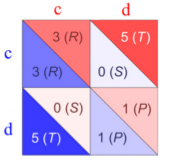
\includegraphics[height=3cm]{./pd.png}
\end{center}


El dilema del prisionero iterado, consiste en sucesivas partidas jugadas por, digamos X e Y.
Aquí los jugadores podrían basar sus jugadas en las jugadas anteriores.Sería natural pensar que el jugador que es
capaz de recordar más jugadas, podría confeccionar una estrategias más eficiente y así llevar ventaja.
Se va a probar luego, que esto no es así, y que solo importa la última jugada. Es por eso que las estrategias seran elaboradas
a partir de el último resultado, sin pérdida de generalidad.
Es decir, cada jugador va a basar su estrategia en el resultado xy $\in$ (cc,cd,dc,dd) donde c significa cooperar y d, no cooperar 
(defect en inglés). La estrategia de X, p=($p_1,p_2,p_3,p_4$) son las probabilidades de cooperar en cada una de las situaciones 
anteriores. En forma análoga, la estrategia de Y es q=($q_1,q_2,q_3,q_4$) visto desde su perspectiva yx $\in$ (cc,cd,dc,dd).

\section{Resultados}
\subsection{Estrategias de determinante cero}
Si bien es posible realizar una simulación del juego, movimiento por movimiento,uno podría evitar esto, con una matriz de
de transición de Markov.Esta matriz es generada a partir de las estrategias p y q.
$$M=
\begin{bmatrix}
 p_1 q_1 &p_1(1-q_1) &(1-p_1)q_1 &(1-p_1)(1-q_1)\\
 p_2 q_3 &p_2(1-q_3) &(1-p_2)q_3 &(1-p_2)(1-q_3)\\
 p_3 q_2 &p_3(1-q_2) &(1-p_3)q_2 &(1-p_3)(1-q_2)\\
 p_4 q_4 &p_4(1-q_4) &(1-p_4)q_4 &(1-p_4)(1-q_4)\\
\end{bmatrix}
$$
El valor $M_{ij}$ representa la probabilidad de pasar de un estado i a un estado j donde, i,j estan asociados a una 
estrategia en (cc,cd,dc,dd), según la perspectiva de cada jugador.
Por ejemplo, $M_{32}$ representa la probabilidad de pasar de un estado dc a cd.
Un vector estacionario v es aquel tal que:
\begin{center}
$v^T M = v^T$
\end{center}
Es decir, un autovector (a izquierda) asociado al autovalor 1.
Con v y el vector de pagos asociado a cada jugador, uno puede calcular el resultado del juego.

Dado que M tiene un autovector asociado al autovalor 1, la matriz M':=M-I es singular y por ende, de 
determinante cero.
Si se aplica la regla de Cramer a la matriz M', se obtiene
\begin{center}
$Adj(M')M' = det(M')I=0$
\end{center}
Sea A:=Adj(M'), entonces por la igualdad anterior, tenemos que:
\begin{center}
$AM'=A(M-I)=0 => AM=A$
\end{center}
Es decir, que el elemento 
\begin{center}
$(AM)_{ij}=\sum_{k=1}^4 A_{ik} M_{kj} = A_{ij}$
\end{center}
Ahora, sea w la n-esima fila de A.
\begin{center}
$w:=(w_1,w_2,w_3,w_4)=(A_{n1},A_{n2},A_{n3},A_{n4})$
\end{center}
Entonces, el j-esimo elemento del vector (w M) es,
\begin{center}
$(w M)_j=\sum_{k=1}^4 w_k M_{kj} =\sum_{k=1}^4 A_{nk} M_{kj} = A_{nj}=w_j$
\end{center}
Es decir que w M= w, por ende, w es proporcional a v.
Dado que n es arbitrario, se puede concluir que cada fila de Adj(M') es proporcional a v

 \section{Bibliografía}
  \begin{thebibliography}{1}
  \end{thebibliography}


\end{document}

